\begin{example}
	\index{Example: Bayesian decision theory}
	\emph{Consider a discrete action space with an observation $X=x$ and available data $D$. Picking a class corresponds to an action, so classification can be viewed as a game against nature, where nature has picked the true class and the robot has to pick a class as well. Suppose there are only two classes and the cost function is defined by the matrix}
	\begin{center}
		\begin{tabular}{ c  c  c  c }
			&& $S$& \\
			&& $s_1$ & $s_2$  \\
			\cline{3-4}
			$U(x)$ & $u_1$& \multicolumn{1}{|l}{$0$} &\multicolumn{1}{l|}{$\lambda_{12}$}  \\
			& $u_2$& \multicolumn{1}{|l}{$\lambda_{21}$} & \multicolumn{1}{l|}{0} \\
			\cline{3-4}
		\end{tabular}
	\end{center}
	\begin{enumerate}
		\item \emph{Show that the decision $u$ that minimizes the expected loss is equivalent to setting a probability threshold $k$ and predicting $U(x)=u_1$ if $p(S=s_2|x,D,I) < k$ and $U(x)=u_2$ if $p(S=s_2|x,D,I)\geq k$. What is $k$ as a function of $\lambda_{12}$ and $\lambda_{21}$?}\newline
		
		The conditional expected cost
		\begin{equation}
			\begin{split}
				\mathbb{E}_{S|X}[C(u, S)|x,D,I] & = \sum_sC(u,S=s)p(S=s|x,D,I)\\
				& = C(u,S=s_1)p(S=s_1|x,D,I)\\
				& \quad+C(u,S=s_2)p(S=s_2|x,D,I)\\
			\end{split}
		\end{equation}
		For the different possible actions
		\begin{equation}
			\begin{split}
				\mathbb{E}_{S|X}[C(u_1, S)|x,D,I] &= \lambda_{12}p(S=s_2|x,D,I),\\
				\mathbb{E}_{S|X}[C(u_2, S)|x,D,I] &= \lambda_{21}p(S=s_1|x,D,I),\\
			\end{split}
		\end{equation}
		$U(x)=u_1$ iff
		\begin{equation}
			\mathbb{E}_{S|X}[C(u_1,S)|x,D,I]<\mathbb{E}_{S|X}[C(u_1,S)|x,D,I])
		\end{equation}
		meaning
		\begin{equation}
			\begin{split}
				\lambda_{12}p(S=s_2|x,D,I)&<\lambda_{21}p(S = s_1|x,D,I)\\
				&=\lambda_{21}(1-p(S =s_2|x,D,I))
			\end{split}
		\end{equation}
		meaning $U(x) = u_1$ iff
		\begin{equation}
			p(S=s_2|x,D,I)<\frac{\lambda_{21}}{\lambda_{12}+\lambda_{21}}=k
		\end{equation}
		
		
		\item \emph{Show a loss matrix where the threshold is $0.1$.}\newline
		
		$k = \frac{1}{21}=\frac{\lambda_{21}}{\lambda_{12}+\lambda_{21}} \Rightarrow \lambda_{12}=9\lambda_{21}$ yielding the loss matrix
		
		\begin{center}
			\begin{tabular}{ c  c  c  c }
				&& $S$& \\
				&& $s_1$ & $s_2$  \\
				\cline{3-4}
				$U(x)$ & $u_1$& \multicolumn{1}{|l}{$0$} &\multicolumn{1}{l|}{$9\lambda_{21}$}  \\
				& $u_2$& \multicolumn{1}{|l}{$\lambda_{21}$} & \multicolumn{1}{l|}{0} \\
				\cline{3-4}
			\end{tabular}
		\end{center}
		
		You may set $\lambda_{21}=1$ since only the relative magnitude is important in relation to making a decision.
		
	\end{enumerate}
	
	
\end{example}


\begin{example}
	\index{Example: Bayesian decision theory}
	\emph{In many classification problems one has the option of assigning $x$ to class $k\in K$ or, if the robot is too uncertain, choosing a reject option. If the cost for rejection is less than the cost of falsely classifying the object, it may be the optimal action. Define the cost function as follows}
	\begin{equation}
		C(u,s)=\begin{cases}
			0 & \text{if correct classification ($u=s$)}\\
			\lambda_r & \text{if reject option $u=$ reject}\\
			\lambda_s & \text{if wrong classification ($u\neq s$)}\\
		\end{cases}.
	\end{equation}
	
	\begin{enumerate}
		\item \emph{Show that the minimum cost is obtained if the robot decides on class $u$ if $p(S=u|x,D,I)\geq p(S\neq u|x,D,I)$ and if $p(S=u|x,D,I)\geq 1-\frac{\lambda_r}{\lambda_s}$.}\newline
		
		The conditional expected cost if the robot does not pick the reject option, meaning $u\in \mathbb{U}\setminus\text{reject}$
		\begin{equation}
			\begin{split}
				\mathbb{E}_{S|X}[C(u, S)|x,D,I] & = \sum_s C(u,S=s)p(S=s|x,D,I)\\
				&= \sum_{s\neq u}\lambda_sp(S=s|x,D,I)\\
				&= \lambda_s(1-p(S=u|x,D,I))
			\end{split}
			\label{eq:cost1}
		\end{equation}
		where for the second equality it has been used that the cost of a correct classification is $0$, so the case of $S=u$ does not enter the sum. For the third equality it has been used that summing over all but $S=u$ is equal to $1-p(S=u|x,D,I)$. The larger $p(S=u|x,D,I)$, the smaller loss (for $\lambda_s>0$), meaning the loss is minimized for the largest probability. The conditional expected loss if the robot picks the reject option
		\begin{equation}
			\begin{split}
				\mathbb{E}_{S|X}[C(\text{reject}, S)|x,D,I]&= \lambda_r\sum_sp(S=s|x,D,I)\\
				&=\lambda_r.
			\end{split}
			\label{eq:cost2}
		\end{equation}
		Equation \eqref{eq:cost1} show picking $\arg\max_{u\in \mathbb{U}\setminus \text{reject}} p(S=u|x,D,I)$ is the best option among classes $u\neq \text{reject}$. To be the best option overall, it also needs to have lower cost than the reject option. Using equations \eqref{eq:cost1} and \eqref{eq:cost2} yields
		\begin{equation}
			(1-p(S=u|x,D,I))\lambda_s< \lambda_r
		\end{equation}
		meaning
		\begin{equation}
			p(S=u|x,D,I)\geq 1-\frac{\lambda_r}{\lambda_s}.
		\end{equation}
		
		\item \emph{Describe qualitatively what happens as $\frac{\lambda_r}{\lambda_s}$ is increased from $0$ to $1$.}\newline
		
		$\frac{\lambda_r}{\lambda_s}=0$ means rejection is rated as a successful classification -- i.e. no cost associated -- and this become the best option (rejection that is) unless $p(y=j|x)=1$, corresponding to knowing the correct class with absolute certainty. In other words; in this limit rejection is best unless the robot is certain of the correct class. $\frac{\lambda_r}{\lambda_s}=1$ means rejection is rated a misclassification -- i.e. $\lambda_r=\lambda_s$ -- and thus and "automatic cost". Hence, in this case rejection is never chosen. In between the limits, an interpolation of interpretations apply.
	\end{enumerate}
\end{example}



\begin{example}
	\paragraph{Setup:} Consider a farmer who wishes to retire and therefore would like to sell their set of live animals. For simplicity, assume that animals make up a simple group and a given person can either be interested in purchasing an animal or not -- the simplfication consist of not differentiating between different animal types. In order to sell their animals, the farmer needs to contact people with a sale in mind. For simplicity, the contact will be assumed to be via a telephone call only. The farmer can call (or not) with the intent to sell an animal to the recepient of the call. The recepient of the call can (or not) be interesed in purchasing an animal (Natures decision). Let $\Omega_U$ denote the set of the farmers actions and $\Omega_S$ the set of Natures actions, then
	\begin{equation}
		\begin{split}
			\Omega_U &= \{u_1 = \text{call}, u_2 = \text{don't call}\},\\
			\Omega_S &= \{s_1 = \text{interested}, s_2 = \text{not interested}\}.
		\end{split}
	\end{equation}
	A nuisance for the contacted people is associated to the call which is represented by the abstract monetary loss, $\lambda\in \mathbb{R}^+$. The degree to which people are annoyed by a sales call is independent in general and the monetary loss represents the average animosity generated and the associated moneraty loss connected to a worsened reputation. Aside from the nuisance associated with a sales call, there is also a moneraty reward for a successfull sale, $\psi$.	If the farmer cannot sell his animals, he will have them terminated with no associated cost in order not to spend additional time or money on them. Given these assumptions, the cost function can be represented by the matrix
	\begin{center}
		\begin{tabular}{  c  c  c }
			& $s_1=$ Interested & $s_2=$ Not interested  \\
			\cline{2-3}
			 $u_1 =$ Call& \multicolumn{1}{|l}{$\lambda-\psi$} &\multicolumn{1}{l|}{$\lambda$}  \\
			 $u_2=$ Don't call& \multicolumn{1}{|l}{$0$} & \multicolumn{1}{l|}{0} \\
			\cline{2-3}
		\end{tabular}
	\end{center}
	The farmer has available to them observations $X=x$ that contain information regarding the decesion Nature is going to make, $S=s$. The farmer also have a collection of past observations and resulting decisions of Nature, i.e. $D= \{(X=x_1,S=s_1),(X=x_2,S=s_2),\dots (X=x_n,S=s_n)\}= D_s\times D_s$. 
	
	\paragraph{Optimal decision rule:} The optimal decision for the farmer to call the $i$'th person can then be written viz
	\begin{equation}
		U^*(x) = \arg\min_{U(x)} \mathbb{E}_{S|X}[C(U(x), S)|X=x,D,I],
	\end{equation}
	where
	\begin{equation}
		\mathbb{E}_{S|X}[C(U(x), S)|X=x,D,I] = \sum_{s\in \mathbb{S}} C(U(x),s) p(S=s|X=x,D,I).
	\end{equation}
	Writing out the conditional expectation
	\begin{equation}
		\begin{split}
			\mathbb{E}[C(u_1, S)] & = \sum_sC(u_1,s)p(s)\\
			& = C(u_1,s_1)p(s_1|x,D,I) + C(u_1,s_2)p(s_2|x,D,I)\\
			& = (\lambda-\psi)p(s_1|x,D,I) + \lambda_i p(s_2|x,D,I),\\
			\mathbb{E}[C(u_2, S)] & = \sum_sC(u_2,s)p(s|x,D,I)\\
			& = C(u_2,s_1)p(s_1|x,D,I) + C(u_2,s_2)p(s_2|x,D,I),\\
			&=0
		\end{split}
	\end{equation}
	where the notation has been compressed to fit the equations to the page. The optimal decision rule $U^*(x)$ can be implicitly specified as picking $u_1$ (call) iff $\mathbb{E}_{S|X}[C(u_1, S)|x,D,I]<\mathbb{E}_{S|X}[C(u_2, S)|x,D,I]$, corresponding to picking $u_1$ (call) iff
	\begin{equation}
		(\lambda-\psi)p(S= s_1|x,D,I) + \lambda p(S= s_2|x,D,I) <0
	\end{equation}
	Since $p(S= s_1|x,D,I) +p(S= s_2|x,D,I) = 1$
	\begin{equation}
		\frac{\lambda}{\psi} < p(S= s_1|x,D,I)
		\label{eq:decision_rule}
	\end{equation}
	meaning the farmer should call (action $u_1$) iff the probability for the recepient of the call to be interested in at least one animal is larger than the penalty of calling divided by the gain of calling. 
	
	\paragraph{The Probability:} \EQref{eq:decision_rule} implicitly specify the decision rule for the farmer. $\lambda,\psi$ is assumed specified, so only the probability $p(S= s_1|x,D,I)$ remain to be specified. Suppose now a model, $f: \Omega_W\times \Omega_X\mapsto[0,1]$, with associated parameters $w\in \Omega_W$, that estimates Nature's actions $S$ based on observed data $X$ is introduced. Using marginalization and assuming independence 
	\begin{equation}
		\begin{split}
			p(S= s|x,D,I) &= \int p(S= s,w|x,D,I) dw \\
			& = \int p(S= s|x,w,D,I)  p(w|x,D,I)dw \\
			& = \int p(S= s|x,w,I)  p(w|D,I)dw. \\
		\end{split}
		\label{eq:q5}
	\end{equation}
	Combining \EQref{eq:q5} and \EQref{f_dist2}
	\begin{equation}
		\begin{split}
			p(S= s|x,D,I) & = \int f_{S = s}(w,x)  p(w|D,I)dw \\
			& = \mathbb{E}[f_{S = s}(w,x)|D,I].\\
		\end{split}
	\end{equation}
	From Bayes theorem \index{Bayes theorem}
	\begin{equation}
		p(w|D,I) =\frac{p(D_s|D_x,w,I)p(w|D_x,I)}{p(D_s|D_x,I)},
	\end{equation}
	where $p(w|D_x,I) = p(w|I)$. Assuming the distribution over $w$ is normally distributed with zero mean and a precision described by a hyperparameter, $\lambda$, 
	\begin{equation}
		p(w|I) = \int p(w|\lambda,I)p(\lambda|I)d\lambda.
		\label{eq:lambda}
	\end{equation}
	The precision is constructed as a wide gamma distribution so as to approximate an objective prior
	\begin{equation}
		p(w|\lambda,I)p(\lambda|I)
		= \prod_{q=1}^{\tilde{n}} \frac{\lambda_q^\frac{n_q}{2}}{(2\pi)^\frac{n_q}{2}}e^{-\frac{\lambda_q}{2}\sum_{l=1}^{n_q}w_l^2}\frac{\beta_q^{\alpha_q}}{\Gamma(\alpha_q)}\lambda_q^{\alpha_q-1}e^{-\beta_q \lambda_q}
		\label{eq:prior}
	\end{equation}
	Assuming the past actions of Nature are independent and identically distributed, the likelihood can be written 
	\begin{equation}
		\begin{split}
			p(D_s|D_x,w,I) &=\prod_{i=1}^{n}p(S = s_i|X = x_i,w,I)\\
			&=\prod_{i=1}^{n}f_{s_i}(w,x_i).\\
		\end{split}
		\label{lik}
	\end{equation}
	Aside from the specification of the model $f$, $p(S= s|x,D,I)$ is at this point fully specified and can be approximated by HMC similarly to the regression case. In this case, the model can be represented by the Hamiltonian 
	\begin{equation}
		H \equiv  \sum_{q}\sum_{l}\frac{p_{l}^2}{2m_{l}}-\ln(p(w,\lambda|D,I))+const
		\label{ham3}
	\end{equation}
	where
	\begin{equation}
		p(w|D,I) = \int d\lambda p(w,\lambda|D,I).
	\end{equation}
	Using \EQref{eq:q5}-\EQref{lik} in \EQref{ham3} yields the Hamiltonian
	\begin{equation}
		\begin{split}
			H&=\sum_{q=1}^{\tilde{n}}\sum_{l=1}^{n_q}\frac{p_{l}^2}{2m_{l}}-\sum_{i=1}^{n}\ln(f_{s_i}(w,x_i))+\text{const}\\
			&\quad+\sum_{q=1}^{\tilde{n}}\bigg(\ln(\Gamma(\alpha_q))-\alpha_q\ln(\beta_q)+(1-\alpha_q)\ln(\lambda_q)+\beta_q\lambda_q\\
			&\qquad \qquad+\frac{n_q}{2}(\ln(2\pi)-\ln(\lambda_q))+\frac{\lambda_q}{2}\sum_{l=1}^{n_q}w_l^2\bigg)\\
		\end{split}.
		\label{ham2}
	\end{equation}
	
	\paragraph{Simple model:} Let
	\begin{equation}
		f_{S = s}(w,x_i) = \frac{e^{b_s+\sum_{q}a_{sq}x_{iq}}}{\sum_{k\in \mathbb{S}}e^{b_k+\sum_{q}a_{kq}x_{iq}}},
		\label{eq:f1}
	\end{equation}
	where $w = \{b,a\}$.
	
	\paragraph{Manual HMC:}	The Hamiltonian is given by
	\begin{equation}
		\begin{split}
			H&=\sum_{q=1}^{2}\sum_{l=1}^{2}\frac{p_{ql}^2}{2m_{ql}}-\sum_{i=1}^{n}\ln(f_{s_i}(w,x_i))\\
			&\quad+\ln(\Gamma(\alpha_a))-\alpha_a\ln(\beta_a)+(1-\alpha_a)\ln(\lambda_a)+\beta_a\lambda_a\\
			&\qquad \qquad+\frac{1}{2}(\ln(2\pi)-\ln(\lambda_a))+\frac{\lambda_a}{2}\sum_{j,q}a_{jq}^2\\
			&\quad+\ln(\Gamma(\alpha_b))-\alpha_b\ln(\beta_b)+(1-\alpha_b)\ln(\lambda_b)+\beta_b\lambda_b\\
			&\qquad \qquad+\frac{1}{2}(\ln(2\pi)-\ln(\lambda_b))+\frac{\lambda_b}{2}\sum_{j}b_j^2\\
		\end{split}
	\end{equation}
	$\lambda_j$ is positive definite. In order to uphold this numerically, let $\lambda_j = e^{\tau_j}$. When making this transformation, the integration measure of \EQref{eq:lambda} has to be transformed as well. This proceeds viz
	\begin{equation}
		d\lambda_j = \lambda_jd\tau_j,
	\end{equation}
	meaning effectively $\lambda_j$ is multiplied on $p(w,\lambda|D,I)$ such that $H \rightarrow H-\ln(\lambda_j)$. This means
	\begin{equation}
		(1-\alpha_j)\ln(\lambda_j)\in H \Rightarrow -\alpha_j \ln(\lambda_j).
	\end{equation}
	Additionally, it is convenient to pick out the $s_i$ via a one-hot target vector such that
	\begin{equation}
		\begin{split}
			H&=\sum_{q=1}^{2}\sum_{l=1}^{2}\frac{p_{ql}^2}{2m_{ql}}-\sum_{j\in \mathbb{S}}\sum_{i=1}^{n}s_{ij}\ln(f_{j}(w,x_i))\\
			&\quad+\ln(\Gamma(\alpha_a))-\alpha_a\ln(\beta_a)-\alpha_a\tau_a+\beta_ae^{\tau_a}\\
			&\qquad \qquad+\frac{1}{2}(\ln(2\pi)-\tau_a)+\frac{e^{\tau_a}}{2}\sum_{j,q}a_{jq}^2\\
			&\quad+\ln(\Gamma(\alpha_b))-\alpha_b\ln(\beta_b)-\alpha_b\tau_b+\beta_be^{\tau_b}\\
			&\qquad \qquad+\frac{1}{2}(\ln(2\pi)-\tau_b)+\frac{e^{\tau_b}}{2}\sum_{j}b_j^2\\
		\end{split}
	\end{equation}
	
	The derivatives are needed for the HMC algorithm
	\begin{equation}
		\frac{\partial H}{\partial a_{ml}} = -\sum_{i,j}\frac{s_{ij}}{f_{ij}}\frac{\partial f_{ij}}{\partial a_{ml}}+e^{\tau_a}a_{ml},\\
	\end{equation}
	\begin{equation}
		\begin{split}
			\frac{\partial f_{ij}}{\partial a_{ml}} & = \frac{e^{b_j+\sum_{q_1}a_{jq_1}x_{iq_1}}}{\sum_{k\in \mathbb{S}}e^{b_k+\sum_{q_2}a_{kq_2}x_{iq_2}}}\sum_{q_3}\delta_{jm}\delta_{q_3l}x_{iq_3}\\
			&\qquad-\frac{e^{b_j+\sum_{q_4}a_{jq_4}x_{iq_4}}}{(\sum_{k\in \mathbb{S}}e^{b_k+\sum_{q_5}a_{kq_5}x_{iq_5}})^2}\sum_{k'\in \mathbb{S}}e^{b_{k'}+\sum_{q_6}a_{k'q_6}x_{iq_6}}\sum_{q_7}\delta_{k'm}\delta_{q_7l}x_{iq_7}\\
			& = f_{ij}\delta_{jm}x_{il}- f_{ij}f_{im}x_{il}
		\end{split}
	\end{equation}
	where it has been used that
	\begin{equation}
		\frac{\partial a_{jq_3}}{\partial a_{ml}} = \delta_{jm}\delta_{q_3l}
	\end{equation}
	
	\begin{equation}
		\begin{split}
			\frac{\partial H}{\partial a_{ml}} &= -\sum_{i,j}\frac{s_{ij}}{f_{ij}}(f_{ij}\delta_{jm}x_{il}- f_{ij}f_{im}x_{il})+e^{\tau_a}a_{ml}\\
			& = \sum_ix_{il}(f_{im}-s_{im})+e^{\tau_a}a_m\\
		\end{split}
	\end{equation}
	\begin{equation}
		\frac{\partial H}{\partial b_m} = \sum_i(f_{im}-s_{im})+e^{\tau_b}b_m.
	\end{equation}
	\begin{equation}
		\frac{\partial H}{\partial \tau_m} = -\alpha_m+\beta_me^{\tau_m}-\frac{1}{2}+\frac{e^{\tau_m}}{2}\sum_jm_j^2.
	\end{equation}
	
	The masses for the HMC algorithm can be set by approximating the second order derivatives as fixed. Let
	\begin{equation}
		\begin{split}
			\frac{\partial^2 H}{\partial a_{ml}^2} &= \sum_ix_{il}\frac{\partial f_{im}}{\partial a_{ml}}+e^{\tau_a}\\
			& =\sum_ix_{il}^2f_{im}( 1- f_{im})+e^{\tau_a}\\
		\end{split}
	\end{equation}
	then taking $x_{il}^2\sim 1, f_{im}\sim \frac{1}{2}$ and any parameter $\sim 0$, meaning $e^{\tau_a} \sim 1$ yield the mass approximation
	\begin{equation}
		\begin{split}
			m_{ml}^{(a)} &\sim \frac{\partial^2 H}{\partial a_{ml}^2}\bigg|_{\text{fixed approximation}}\\
			& \sim N\cdot 1^2\cdot \frac{1}{2}(1-\frac{1}{2})+1\\
			&=\frac{N}{4} +1,
		\end{split}
	\end{equation}
	where $N$ is the number of data samples in $D_x$. Similarly
	\begin{equation}
		\begin{split}
			\frac{\partial^2 H}{\partial b_m^2} &= \sum_i\frac{\partial f_{im}}{\partial a_{ml}}+e^{\tau_b}\\
			& =\sum_if_{im}( 1- f_{im})+e^{\tau_b},
		\end{split}
	\end{equation}
	meaning (since $x_{il}^2\sim 1$)
	\begin{equation}
		\begin{split}
			m_{ml}^{(a)} &\sim \frac{\partial^2 H}{\partial b_{m}^2}\bigg|_{\text{fixed approximation}}\\
			& m_{ml}^{(b)}.
		\end{split}
	\end{equation}
	The precision parameter
	\begin{equation}
		\frac{\partial^2 H}{\partial \tau_q^2} = \beta_qe^{\tau_q}+\frac{e^{\tau_q}}{2}\sum_jq_j^2.
	\end{equation}
	Take $\beta_q = 3$, then
	\begin{equation}
		\begin{split}
			m_{q}^{(\tau)} &\sim \frac{\partial^2 H}{\partial \tau_{q}^2}\bigg|_{\text{fixed approximation}}\\
			&\sim 3.
		\end{split}
	\end{equation}
	
	
	
	
	\paragraph{Data:} Take $x=(\text{area},\text{number of animals})^T$ and $s=$ 2d one-hot vector, with $\dim(D)=1000$. $D$ is split into two sets $D^{(\text{training})}$ and $D^{(\text{test})}$, with $\dim(D^{(\text{training})})=\gamma\dim(D)$ and $\dim(D^{(\text{test})})=(1-\gamma)\dim(D)$ and $\gamma=0.6$. $D^{(\text{training})}$ will be used to train the model and $D^{(\text{test})}$ to evaluate the quality of the trained model. The underlying truth of Nature (unbeknownst to the model) is that an animal will be purchased iff
	\begin{equation}
		\text{total area}- 3.2\cdot\text{number of animals}\geq 3.2.
		\label{eq:nature}
	\end{equation}
	
	\paragraph{Training:} Using $D^{(\text{training})}$ as input, the algorithms the algorithms are trained for $2000$ iterations. The first $500$ iterations are taken as burn in to be conservative. The coefficients, $w$, for iterations $[500,2000]$ are used to make a model prediction viz
	\begin{equation}
		p(S= s|x,D,I)=\frac{1}{1500}\sum_{i=500}^{2000}f(w_i,x)
	\end{equation}
	The accuracy of the modeled probabilities can be gauged by considering the case where $\psi=2\lambda$ such that the decision rule (\EQref{eq:decision_rule}) becomes
	\begin{equation}
		\frac{1}{2} < p(S= s_1|x,D,I),
		\label{eq:decision_rule2}
	\end{equation}
	and the classification is driven by the probabilities alone. 
	
	
	\paragraph{PyMC HMC Algorithm:} PyMC is a probabilistic programming library for Python that allows users to build Bayesian models with a Python API and fit them using Markov Chain Monte Carlo methods \href{https://www.pymc.io/welcome.html}{PyMC link}. Using this API it is possible to create, train and test a PyMC-equivalent of the model described in the previous sections. The general approach to building a model using PyMC consists of stating the data generating process, specifying a likelihood, and related prior distributions for any parameters involved. While modeling the data generating process and framing the statistical problem correctly are never completely trivial and require some effort from the user it is rather straight forward to perform the Markov Chain Monte Carlo sampling with PyMC. The user do not need to do any calculations related to the Hamiltonian Monte Carlo method nor do they need to specifically handle any integrals. In addition, there is a range of predefined probability distributions both discrete and continuous readily available in the library such as the Gamma (figure \ref{fig:gamma}) and Normal distribution used for modeling the priors.
	\begin{figure}[H]
		\centering
		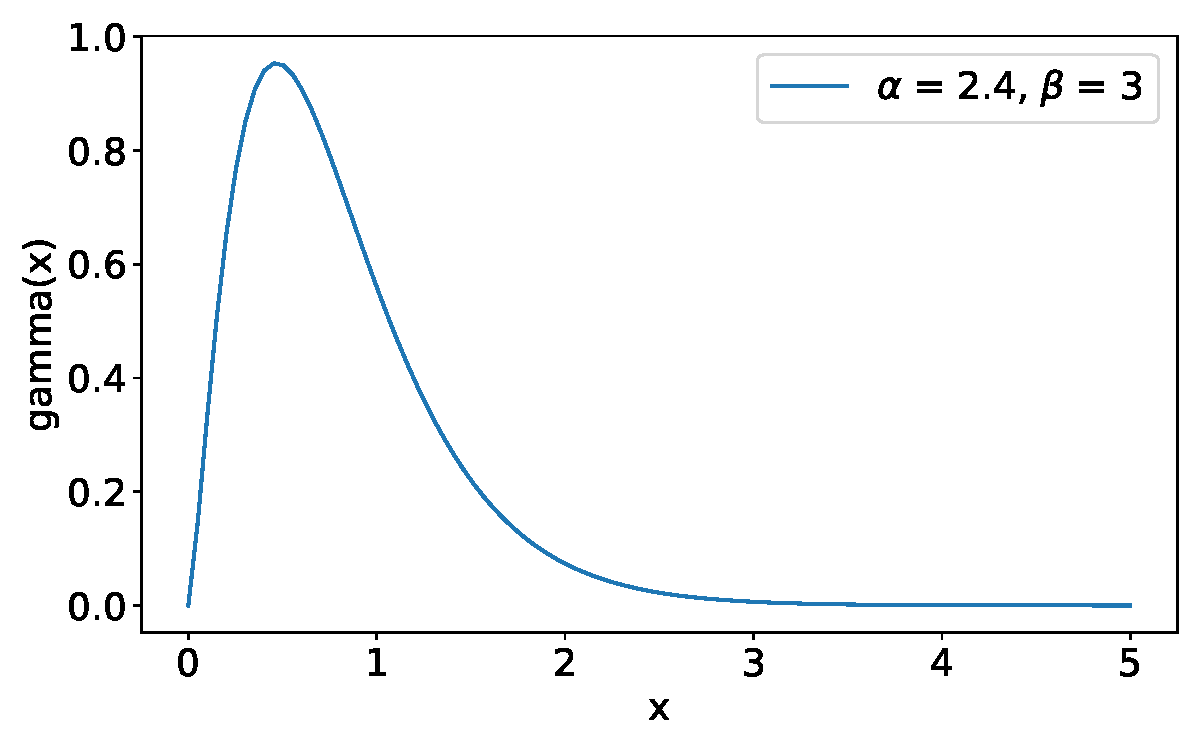
\includegraphics[width = 1\textwidth]{figures/gamma_dist.pdf}
		\caption{Plot of Gamma probability distribution used as priors for the precision parameters in Normal distributions.}
		\label{fig:gamma}
	\end{figure}
	The python code in \algref{algo:pymc_model} shows how the simple model can be declared using PyMC. All models in PyMC are declared using a "with pm.Model() as modelname"-statement, where pm is the abbreviated form of the PyMC package. Within this statement at range of random variables, data and their relations can be declared. The syntax for declaring a random variable by its probability distribution (such as pm.Normal) is to pass a name for the random variable as a string for the first argument. The rest of the arguments are typically values for the parameters specific to the distribution. PyMC random variables can often be used for stating parameters in other random variables forming a hierarchy of distributions as is the case for the precision variables used to model the variance for the normally distributed parameters a and b (see \EQref{eq:f1}) with zero mean. In the code example, these parameters are then combined deterministically with $D_x$ to constitute the data generating process of the simple model. $D_x$ is declared as a PyMC mutable object so that it will be possible later to change the values to generate predictions. As a last step the likelihood is declared. In PyMC this is the step where the relationship between the observed conditional ($D_s$) data and parameters is stated. As the output is the probabilities for the two classes a Multinomial distribution with the number of independent trials (n) equal to 1 is used as the likelihood. 
	
	\begin{algorithm}[H]
		\caption{PyMC Python Code}
		\begin{python}
			import pymc as pm
			import numpy as np
			with pm.Model() as classifier_model:
			covars = pm.MutableData('covars',data_x_training) 
			# Priors for precision
			precision_a = pm.Gamma('precision_a', alpha=2.4, beta=3)
			precision_b = pm.Gamma('precision_b', alpha=2.4, beta=3)
			# Priors for parameters
			param_a = pm.Normal('param_a', 
			0, 
			sigma=1/np.sqrt(precision_a),
			shape=(2,2))
			param_b = pm.Normal('param_b', 
			0, 
			sigma=1/np.sqrt(precision_b),
			shape=(2,))
			# Data generating process
			T = pm.Deterministic('T', pm.Math.exp(param_b + pm.math.dot(covars, param_a.T)))
			class_conditional_probability = pm.Deterministic('class_conditional_probability', T/T.sum(axis=1, keepdims=True))
			# Likelihood
			obs = pm.Multinomial('obs', n=1, p=class_conditional_probability, observed=data_s_training, shape=class_conditional_probability.shape)
		\end{python}
		\label{algo:pymc_model}
	\end{algorithm}
	
	
	After declaring the model it is possible to sample the posterior by calling the pm.sample() method. Burn-in can be controlled by setting the tune argument. The draw argument determines how many samples are being drawn while a number of chains can be run in parallel by setting the chains and cores (computational) arguments. 	
	\begin{algorithm}[H]
		\label{algo:posteriro}
		\caption{PyMC Posterior Python Code}
		\begin{python}
			with classifier_model:
			posterior = pm.sample(tune=512, draws=1024, chains=4, cores=4)
		\end{python}  
	\end{algorithm}
	
	Using the result of drawing samples from the distribution of model parameters (posterior) it is possible to draw from the posterior predictive distribution using the pm.sample\_posterior\_predictive() method. Without changing the input data this is equivalent to obtaining the result of applying the trained model on $D_x^{(\text{training})}$. By changing the input data to $D_x^{(\text{test})}$ using the pm.set\_data() method it is possible to obtain the posterior predictive distribution.
	
	\begin{algorithm}[H]
		\label{algo:posteriro_predictive}
		\caption{PyMC Posterior Python Code}
		\begin{python}
			with classifier_model:
			posterior_predictive = pm.sample_posterior_predictive(posterior)
			pm.set_data({'covars': data_x_test})
			posterior_predictive_test = pm.sample_posterior_predictive(posterior)
		\end{python}
	\end{algorithm}
	
	Using \EQref{eq:decision_rule2} for $D^{(\text{training})}$, the PyMC model correctly classify $598$ of $600$ data points. For $D^{(\text{test})}$, the model correctly classify $398$.
	
	\paragraph{Results: } The HMC algorithm have parameters "step\_scale" and "number\_of\_steps\_scale", which adjust the overall scale of the step lengths and number of steps in pase space. Ideally, the distance between points should be large, so that step scale should be small (what the step length is divided by should be small) and the number of steps should be large. Numerical stability only exist for step\_scale $\gtrsim 5$ (given accurate mass estimation) and thus only the number of steps remain as a variable to tune. In this study step\_scale $=10$ and number\_of\_steps\_scale $=1500$, where the latter is limited by reasonable computation time (to match approximately the pymc computation time). Given these parameters, the manual HMC algorithm misclassify a single training data point
	\begin{equation}
		x^{(\text{training})}_{\text{misclassified 1}} = \begin{pmatrix}
			3.21798365\\ 0\\
		\end{pmatrix}
		\label{eq:misclassified1_training}
	\end{equation}
	and two test data points
	\begin{equation}
		x^{(\text{test})}_{\text{misclassified 1}} = \begin{pmatrix}
			6.40501793\\ 1\\
		\end{pmatrix}, \quad x^{(\text{test})}_{\text{misclassified 2}} = \begin{pmatrix}
			9.60627827\\ 2\\
		\end{pmatrix}.
		\label{eq:misclassified1_test}
	\end{equation}
	With \EQref{eq:nature} in mind, it is clear that the misclassifications of \EQref{eq:misclassified1_training} and \EQref{eq:misclassified1_test} are close to the limit with respect to purchasing an animal.  
	
	
	The PyMC HMC Algorithm obtain misclassify two training data points; \EQref{eq:misclassified1_training} and 
	\begin{equation}
		x^{(\text{training})}_{\text{misclassified 2}} = \begin{pmatrix}
			12.80826256\\ 3\\
		\end{pmatrix}
		\label{eq:misclassified1_training2}
	\end{equation}
	and two test data points (\EQref{eq:misclassified1_test}).
	
	
	\paragraph{Summary and Discussion:} It has been shown how decision theory can be used in conjunction with statistics to make theoretically optimal decisions based on a user specified set of preferences (cost function). Using mock data, a "manual HMC algorithm" written by hand and a standard Python "PyMC HMC algorithm" have been compared. The two yield identical results on test data with the manual model yielding marginally better results on training data. Overall the performace is deemed equivalent both in terms of accuracy and computational speed. The manual HMC algorithm require the user to derive the gradients, write the sampling algorithm in Python and tune the algorith, whereas the latter only require a specification of the model via a standardized PyMC interface. Hence, from a user complexity perspective, the PyMC algorithm has a significant advantage.
\end{example}